\documentclass[12pt]{article}
\usepackage{geometry}
\usepackage{graphicx}
\usepackage{longtable}
\usepackage{dcolumn}
\usepackage{pdflscape}
\usepackage{amsmath}
\usepackage[skip=1ex,bf]{caption}
\usepackage[nottoc,notlot,notlof,numbib]{tocbibind}

\bibliographystyle{abbrv}

\geometry{left=1in,right=1in,top=1in,bottom=1in}

\title{Data-Driven Alternatives to Survey Research}
\author{David deLacoste-Azizi}
\date{May 10, 2018}

\begin{document}

\maketitle

\tableofcontents
 
\listoftables

\listoffigures

\section{Introduction}

Politicians and academics alike have long struggled to perfect a system for predicting the participation of voters at an individual level. The implications for electoral politics are salient: political messages can be tailored to segments of the electorate more likely to actually cast ballots --- and mobilization efforts through direct voter contact or targeted advertising can be focused on constituents that might not otherwise turn out. Furthermore, voting is an essential component of democracy; understanding the factors that encourage people to participate (or not) is an important lens on the underlying institutions. That is, the citizenry's engagement with its government is revealing of that establishment.

Survey research serves as a useful proxy for unadulterated measures of the electorate --- political polling presents a window into public opinion by means of statistical inference. However, this approach has inherent limitations. Connate disparities between the sampling frame and population of interest, whether arising from reliance on respondent self-identification of registration status or systemic, non-random non-response, engender bias in results. Weighting adjustment with auxiliary variables furnishes an imperfect recourse; the demographic or ideological distributions assumed to be ``true'' are typically statistical inferences in their own right. Meanwhile, likely-voter models developed from recent and historical election outcomes and time-series surveys are ill-equipped to compensate for shifts in prevalent views among the public or fluctuations in issue saliency \cite{Traugott:2003aa, Mann:2003aa}.

Furthermore, the decreasing trend in response rates for telephone-based random samples and the accelerating transition from listed landline numbers to unlisted mobile phones have inflated the cost of traditional polling, triggering a resultant movement toward internet-implemented panel surveys. Unfortunately, though such focus groups can inexpensively obtain large numbers of responses, the gulf between sampling frame and population is wider still and the results ever more variable \cite{Zukin:2015aa}.

There are at least two paths forward. The first is the effective incorporation of alternative data sources, including the application of machine learning techniques and so-called ``Big Data.'' These alternative data sources are the focus of this paper. The second is the renovation and refinement of weighting adjustments, which will be imperative for the use of survey research in social science to continue reliably. Enhanced weighting is an area in need of further study; it is conveniently well-suited to the leveraging of techniques from the alternative data strategy.

The use of alternative data sources approached the predictive modeling of voter behavior along a trajectory that is orthogonal to survey research. In stark contrast to the process of collecting information about a random sample drawn from a sampling frame that may differ from the population of interest --- where chance variation can yield significant divergence in representation compared to the population --- techniques which leverage reliable, publicly available data to match each individual in question with demographic, economic, and even personal information enable precision far exceeding that of statistical inference.

In the age of public sharing enabled by social media, individual-level data are not exactly scarce; they are, however, closely guarded by the companies which collect them. As a result, such data are often expensive or otherwise inaccessible to both researchers and campaign professionals. The notable exception of the recent Facebook--Cambridge Analytica scandal has focused national attention on data mining from internet platforms. This strategy is a paradigmatic example of a data-based alternative to survey research: profile information on millions of individuals was combined with voter registration information to identify and target those individuals and their associates.
 
However, data mining on that scale is a highly evolved process and is not universally accessible. While a significant amount of intelligence might be gleaned from public posts on social media sites, the pairing of other publicly available data with the voter file is less expensive and highly attainable. Reducing it to its most basic form, this operation involves pairing individual-level data from any novel source with a state voter file and using that information to target political advertisements, plan direct voter contact, inform campaign strategy, and predict voter behavior \cite{Igielnik:2018aa}.

This paper explores the methodology of alternative data techniques by evaluating the predictive power of the combination of the Philadelphia Voter File and block-level United States Census Bureau data against each of those sources considered individually. Under the assumption that humans are likely to self-sort into similar locations based on both observable and unobservable common characteristics, the expectation is that attaching demographic information from the decennial Census to the voter file boosts predictive performance in modeling voter turnout. 

Using both generalized linear models and deep learning models, information provided by voter registrations alone is moderately effective in predicting the behavior of voters in Philadelphia, Pennsylvania. Census data are somewhat effective when considered alone. The combination of both sources yields a moderately effective predictive model with small improvement over the individual models; this is somewhat supportive of the expectation that combining data from alternative sources increases performance. Additionally, there is evidence in favor of the assumption of assortative habitation.

%\section{Theory and Previous Literature}

\section{Data}

The population of interest is individuals who are eligible to vote. In the models developed for this analysis, the universe is represented by registered voters. As a result of this simplification, non-contemporaneous inferences about the complete population are not valid unless corrected for distributional shifts in the population of registered voters \cite{Brendan:2917aa}.

\subsection{Voter File}
To evaluate these models, the population is constrained to eligible individuals in Philadelphia, Pennsylvania and represented by the Pennsylvania Department of State's Full Voter Export (FVE) for Philadelphia County. 

From the 1,034,518 voters listed in the voter file as of July 2017, the models evaluated only 891,234. To eliminate outliers from missing or incorrect information, 52,403 entries labelled ``Inactive'' by the state are removed, as is one which was missing a birthdate and 372 with registration dates earlier than the associated birthdates. In order to ensure that the model only incorporates information available before the election took place on November 8, 2016, 20,160 registrations submitted after election day are dropped. Similarly, 70,285 registrations updated after that date are removed. Additionally, one voter who would have been underage for the election is not considered; nor are nine people with a common address that could not be placed to a real physical location within the city of Philadelphia.

Table \ref{fvevariables} in the appendix is a list of the 153 original variables from the FVE. The models considered only 14 variables, including the dependent variable indicating participation in the 2016 general election. The variables were recoded or calculated as follows:

\begin{description}
\item [Age on Election Day in 2016:] the difference between the listed date of birth and November 8, 2016 in POSIX time units adjusted for leap intervals and converted to years; standardized to $\mu = 0$ and $\sigma = 1$.
\item [Age when Registered to Vote:] the difference between the listed registration date and the listed date of birth in POSIX time units adjusted for leap intervals and converted to years; standardized to $\mu = 0$ and $\sigma = 1$.
\item [Days Registered by Election Day:] the difference between November 8, 2016 and the listed registration date in POSIX time units converted to days; standardized to $\mu = 0$ and $\sigma = 1$.
\item [Days Between Last Update and E-Day:] the difference between November 8, 2016 and the listed date of last update in POSIX time units converted to days; standardized to $\mu = 0$ and $\sigma = 1$.
\item [Participation in General Elections:] the proportion calculated from the number of the last six general elections in which a voter participated over the number for which that voter was registered.
\item [Registered as Female:] an indicator for a registration with sex recorded as female.
\item [Registered as Male:] an indicator for a registration with sex recorded as male.
\item [Registered as Democrat:] an indicator for a Democratic registration.
\item [Registered as Republican:] an indicator for a Republican registration.
\item [Registered as Independent:] an indicator for an Independent registration.
\item [Phone Number in Registration:] an indicator for a registration with any non-missing value recorded for the phone number.
\item [Phone Number Validated:] an indicator for a registration with a phone number including a valid area code for the United States under the North American Numbering Plan.
\item [Out of State Area Code:] an indicator for a registration with a phone number including an area code that is not assigned to numbers within Pennsylvania.
\item [Out of City Area Code:] an indicator for a registration with a phone number including an area code that is not assigned to numbers within Philadelphia.
\end{description}

Descriptive statistics for these variables can be found in Table \ref{fvestats} in the appendix; additionally, Table \ref{fveunscaledstats} includes descriptive statistics for the continuous variables before scaling and centering operations were used to standardize them. Census data on the addresses included in each block were used to match each voter to the appropriate block.

\subsection{Decennial Census}
The 2010 Decennial Census Summary File 1 contains information for 18,872 blocks ascribed to Philadelphia County. Only 14,871 unique blocks appear in the voter file as some blocks are nonresidential. A large number of tables containing counts of individuals or housing units in each block subdivided into specific demographic strata is available; the models in this exercise evaluate just 65 separate variables from seven tables:

\begin{description}
\item [Average Household Size:] the average household size for each block was reported directly.
\item [Average Family Size:] the average family size for each block was reported directly.
\item [Race:] for each variable within the Race table, the count of individuals per demographic segment was divided by the total number of individuals in the block to create a proportion for comparison to other blocks.
\item [Age by Sex:] for each variable within the Age by Sex table, the count of individuals per demographic segment was divided by the total number of individuals in the block to create a proportion for comparison to other blocks.
\item [Household Type:] for each variable within the Household Type table, the count of individuals per demographic segment was divided by the total number of individuals in the block to create a proportion for comparison to other blocks.
\item [Occupancy Status:] for each variable within the Occupancy Status table, the count of housing units of each type was divided by the total number of housing units in the block to create a proportion for comparison to other blocks.
\item [Tenure:] for each variable within the Tenure table, the count of housing units of each type was divided by the total number of housing units in the block to create a proportion for comparison to other blocks.
\end{description}

Descriptive statistics for all of the variables derived from these tables can be found in Table \ref{censusstats} in the appendix.

\section{Hypotheses and Empirical Tests}
The expectation is that attaching demographic information from the decennial Census to the voter file boosts predictive power and accuracy in modeling voter turnout. This will be tested across two techniques: generalized linear models and deep learning models.

The generalized linear model in the binomial family with the logit link function is a multivariable logistic regression. The deep learning model for classification of a Bernoulli-distributed response is an artificial neural network with three layers of hidden neurons; the first and third layers have 100 neurons while the middle layer has 200.

Three models are developed with each technique through subsets of the combined data. The first subsection considers only the effects of variables from the voter file on individual participation in the 2016 general election. The second considers only the effects of demographic information from the Census on individual participation in the 2016 general election. The third considers the effects of variables from both sources.

To build and evaluate these models, the data are split by random assignment into a set of training data and test data; the assignment is under a distribution that apportions approximately $\frac{2}{3}$ of the entries to the training group and $\frac{1}{3}$ to the test group. Using the H2O data analysis software \cite{Kraljevic:2018aa}, the binomial logit generalized linear model and Bernoulli classification deep learning model are fit over the training data for each of the three subsets to create six models which are distinguishable by the combination of subset and technique.

The resulting models are assessed by calculating predictions on the test data; these predictions are compared with the true values to determine for each model, among other metrics, the Matthews correlation coefficient, the area under the receiver operating characteristic curve, and the accuracy.

As a balanced measure of quality which takes into account true and false positives and negatives \cite{Chicco:2017aa}, the Matthews correlation coefficient ($M$) is used to assess the hypothesis that the inclusion of Census information improves classification performance over the voter file alone. The associated null hypothesis is that there is no difference in performance between the combined model and the model which considered only the voter file; the alternative hypothesis is a difference greater than zero:
$$H_0: M_{\text{Combined}} - M_{\text{FVE Only}} = 0$$
$$H_a: M_{\text{Combined}} - M_{\text{FVE Only}} > 0$$

Additionally, the area under the receiver operating characteristic curve ($A$) is used to examine the underlying assumption that people are likely to live near others with similar voting habits. The null hypothesis for the assumption of assortative habitation is that the area under the ROC curve for the models which considered only Census data is equal to the area of a model which randomly assigned responses ($0.5$); the alternative hypothesis is an area greater than $0.5$:
$$H_0: A_{\text{Census Only}} = 0.5$$
$$H_a: A_{\text{Census Only}} > 0.5$$

\section{Results}

For predicting the behavior of voters in Philadelphia, Pennsylvania, information provided by voter registrations alone is moderately effective: in the generalized linear model, the Matthews correlation coefficient is $0.303$; in the deep learning model, the Matthews correlation coefficient is $0.355$. Census data are somewhat effective when considered alone: in the generalized linear model, the Matthews correlation coefficient is $0.117$; in the deep learning model, the Matthews correlation coefficient is $0.113$. The combination of both sources yields a reasonably effective predictive model: in the generalized linear model, the Matthews correlation coefficient is $0.306$; in the deep learning model, the Matthews correlation coefficient is $0.365$. Figure \ref{mcc} shows the coefficient for each model in a bar chart for comparison.

\begin{figure}
\centering \caption{Matthews Correlation Coefficient by Subset and Technique} \label{mcc}
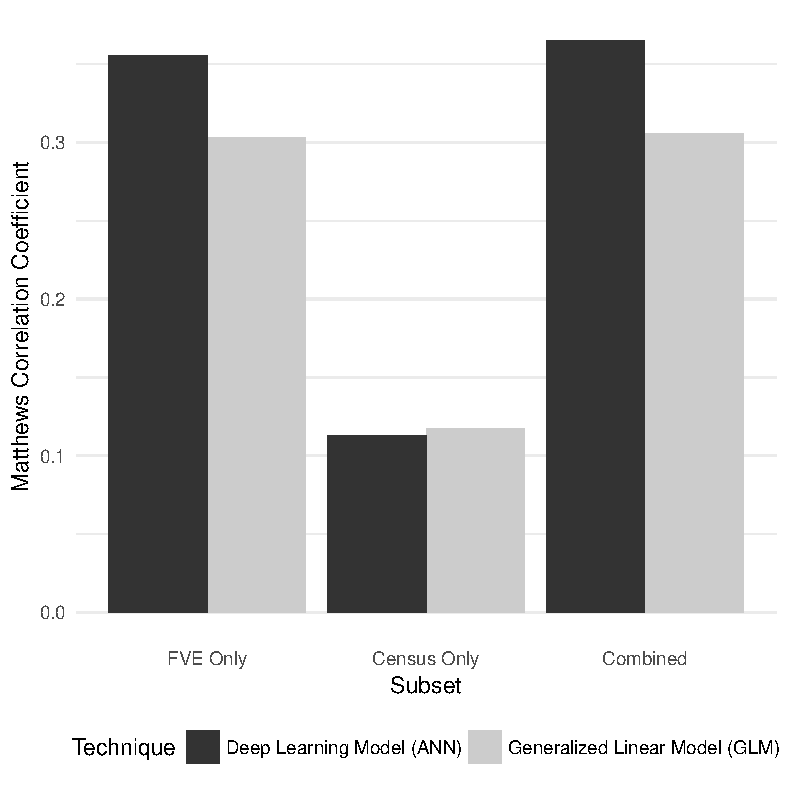
\includegraphics[width=10cm]{Graphic001.pdf}
\end{figure}

The differences between the Matthews correlation coefficient for the combined model and the model considering the voter file alone are $0.002$ for the generalized linear models and $0.01$ for the deep learning models. Since these are both greater than zero, the null hypothesis is rejected in favor of the alternative hypothesis. Unfortunately, without standard errors and confidence intervals, it is unclear whether this difference is statistically significant. While the effect size is quite small in terms of the Matthews correlation coefficient, the magnitude of the effect in terms of voters correctly classified is between $1,000$ and $6,000$; this is a practically significant difference for any campaign.

Additionally, there is evidence in favor of the assumption of assortative habitation. The areas under the receiver operating characteristic curve for the models which only considered Census data are $0.594$ for the generalized linear model and $0.589$ for the deep learning model. Since these are both greater than $0.5$, the null hypothesis that the Census prediction would be no better than random chance is rejected. Though statistical significance cannot be determined, because the area under the ROC curve ranges from 0 to 1, the effect is a practically significant improvement from random guessing. Figure \ref{auroc} shows the area for each model in a bar chart for comparison.

\begin{figure}
\centering \caption{Area Under ROC Curve by Subset and Technique} \label{auroc}
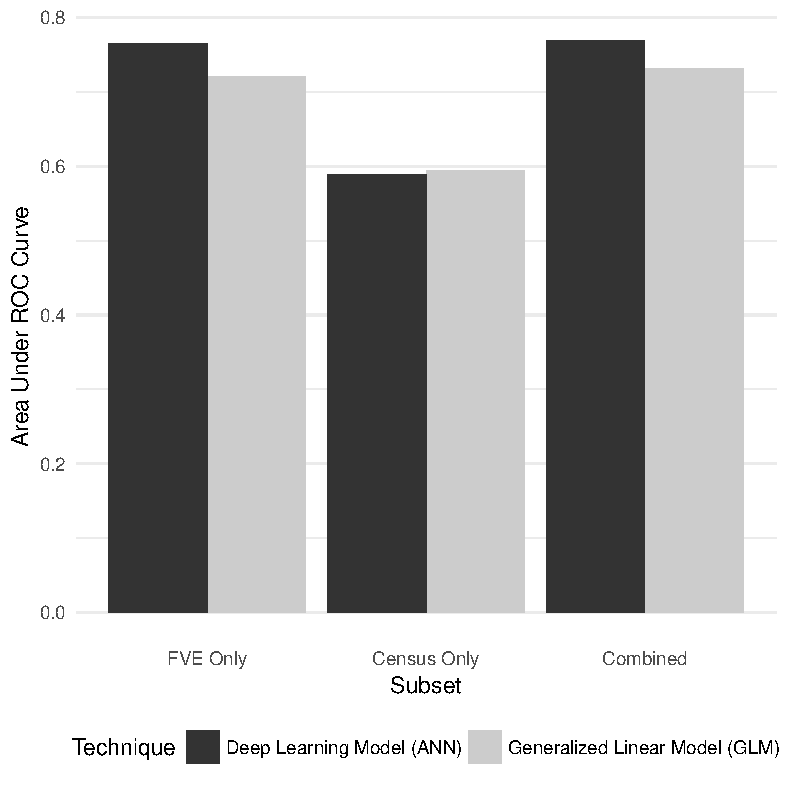
\includegraphics[width=10cm]{Graphic002.pdf}
\end{figure}

Table \ref{modeval} in the appendix presents all of the evaluation metrics available for each model. Figure \ref{accuracy} in the appendix shoes a bar chart of the accuracy for each model; however, since around 75\% of the voters in the dataset participated in 2016 (an unusual rate compared to previous years), the greater proportion of true positives means that accuracy may not be a valid measure of predictive performance. 

The coefficients for the generalized linear models are in Table \ref{glm} in the appendix. An analysis of these coefficients suggests that the most contributory variables on an individual level are previous election participation, an out of city area code, an out of state area code, and partisan registration of any kind. On a block level, the most contributory variables are the proportion of American Indians and Alaska Natives alone, the proportion of Native Hawaiian and Pacific Islanders alone, the proportion of males aged 50 to 54, the proportion of males aged 55 to 59, and the proportion of males aged 40 to 44. Unfortunately, the analysis tool H2O does not calculate standard errors for the coefficients.

\section{Discussion and Conclusion}

It is clear that data that are individual in scope enable significant predictive advantages over aggregate data. However, publicly available data do provide a small improvement in predictive performance which can have a significant impact on the larger scale of a campaign. While useful for predicting behavior on an individual level, these models are limited in evaluation of aggregate outcomes; the mismatch between the population of interest (eligible voters) and the population which is measured (registered voters) is a particularly noteworthy discrepancy since campaigns often focus at least some of their field work on voter registration activities.

Another approach to this analysis involves web-scraping to pair sentiment analysis of social media data with the voter file. This approach maintains a constant ambit and likely yields more significant results; it also directly associates with the data mining operations conducted by both corporations and modern campaigns. 

This paper stops short of evaluating the effectiveness of data-driven approaches in comparison to that of survey research; such a comparison requires the application of a comparable individual-level predictive model built from a traditional survey-based likely-voter model to the same test data. That evaluation is an interesting avenue for further research.

\nocite{*}

\clearpage
\appendix
\section{Appendix}


\begin{table}[!htbp] \centering 
  \caption{Original Variables in the Full Voter Export} 
  \label{fvevariables} 
\small 
\begin{tabular}{@{\extracolsep{5pt}} cl} 
\\[-1.8ex]\hline 
\hline \\[-1.8ex] 
1 & ID Number \\ 
2 & Title \\ 
3 & Last Name \\ 
4 & First Name \\ 
5 & Middle Name \\ 
6 & Suffix \\ 
7 & Gender \\ 
8 & DOB \\ 
9 & Registration Date \\ 
10 & Voter Status \\ 
11 & Status Change Date \\ 
12 & Party Code \\ 
13 & House Number \\ 
14 & House Number Suffix \\ 
15 & Street Name \\ 
16 & Apartment Number \\ 
17 & Address Line 2 \\ 
18 & City \\ 
19 & State \\ 
20 & Zip \\ 
21 & Mail Address 1 \\ 
22 & Mail Address 2 \\ 
23 & Mail City \\ 
24 & Mail State \\ 
25 & Mail Zip \\ 
26 & Last Vote Date \\ 
27 & Precinct Code \\ 
28 & Precinct Split ID \\ 
29 & Date Last Changed \\ 
30 & Custom Data 1 \\ 
31 & District 1 \\ 
32 & District 2 \\ 
33 & District 3 \\ 
34 & District 4 \\ 
35 & District 5 \\ 
36 & District 6 \\ 
37 & District 7 \\ 
38 & District 8 \\   
\hline \\[-1.8ex] 
\end{tabular}
\begin{tabular}{@{\extracolsep{5pt}} cl}
\\[-1.8ex]\hline 
\hline \\[-1.8ex] 
39 & District 9 \\ 
40 & District 10 \\ 
41 & District 11 \\ 
42 & District 12 \\ 
43 & District 13 \\ 
44 & District 14 \\ 
45 & District 15 \\ 
46 & District 16 \\ 
47 & District 17 \\ 
48 & District 18 \\ 
49 & District 19 \\ 
50 & District 20 \\ 
51 & District 21 \\ 
52 & District 22 \\ 
53 & District 23 \\ 
54 & District 24 \\ 
55 & District 25 \\ 
56 & District 26 \\ 
57 & District 27 \\ 
58 & District 28 \\ 
59 & District 29 \\ 
60 & District 30 \\ 
61 & District 31 \\ 
62 & District 32 \\ 
63 & District 33 \\ 
64 & District 34 \\ 
65 & District 35 \\ 
66 & District 36 \\ 
67 & District 37 \\ 
68 & District 38 \\ 
69 & District 39 \\ 
70 & District 40 \\ 
71 & Election 1 Vote Method \\ 
72 & Election 1 Party \\ 
73 & Election 2 Vote Method \\ 
74 & Election 2 Party \\ 
75 & Election 3 Vote Method \\ 
76 & Election 3 Party \\  
\hline \\[-1.8ex] 
\end{tabular}
\end{table} 
\begin{table}[!htbp] \centering 
  \caption*{\textbf{Table \ref{fvevariables} Continued:} Original Variables in the Full Voter Export}
\small 
\begin{tabular}{@{\extracolsep{5pt}} cl}
\\[-1.8ex]\hline 
\hline \\[-1.8ex]  
77 & Election 4 Vote Method \\ 
78 & Election 4 Party \\ 
79 & Election 5 Vote Method \\ 
80 & Election 5 Party \\ 
81 & Election 6 Vote Method \\ 
82 & Election 6 Party \\ 
83 & Election 7 Vote Method \\ 
84 & Election 7 Party \\ 
85 & Election 8 Vote Method \\ 
86 & Election 8 Party \\ 
87 & Election 9 Vote Method \\ 
88 & Election 9 Party \\ 
89 & Election 10 Vote Method \\ 
90 & Election 10 Party \\ 
91 & Election 11 Vote Method \\ 
92 & Election 11 Party \\ 
93 & Election 12 Vote Method \\ 
94 & Election 12 Party \\ 
95 & Election 13 Vote Method \\ 
96 & Election 13 Party \\ 
97 & Election 14 Vote Method \\ 
98 & Election 14 Party \\ 
99 & Election 15 Vote Method \\ 
100 & Election 15 Party \\ 
101 & Election 16 Vote Method \\ 
102 & Election 16 Party \\ 
103 & Election 17 Vote Method \\ 
104 & Election 17 Party \\ 
105 & Election 18 Vote Method \\ 
106 & Election 18 Party \\ 
107 & Election 19 Vote Method \\ 
108 & Election 19 Party \\ 
109 & Election 20 Vote Method \\ 
110 & Election 20 Party \\ 
111 & Election 21 Vote Method \\ 
112 & Election 21 Party \\ 
113 & Election 22 Vote Method \\ 
114 & Election 22 Party \\ 
115 & Election 23 Vote Method \\   
\hline \\[-1.8ex] 
\end{tabular}
\begin{tabular}{@{\extracolsep{5pt}} cl}
\\[-1.8ex]\hline 
\hline \\[-1.8ex] 
116 & Election 23 Party \\ 
117 & Election 24 Vote Method \\ 
118 & Election 24 Party \\ 
119 & Election 25 Vote Method \\ 
120 & Election 25 Party \\ 
121 & Election 26 Vote Method \\ 
122 & Election 26 Party \\ 
123 & Election 27 Vote Method \\ 
124 & Election 27 Party \\ 
125 & Election 28 Vote Method \\ 
126 & Election 28 Party \\ 
127 & Election 29 Vote Method \\ 
128 & Election 29 Party \\ 
129 & Election 30 Vote Method \\ 
130 & Election 30 Party \\ 
131 & Election 31 Vote Method \\ 
132 & Election 31 Party \\ 
133 & Election 32 Vote Method \\ 
134 & Election 32 Party \\ 
135 & Election 33 Vote Method \\ 
136 & Election 33 Party \\ 
137 & Election 34 Vote Method \\ 
138 & Election 34 Party \\ 
139 & Election 35 Vote Method \\ 
140 & Election 35 Party \\ 
141 & Election 36 Vote Method \\ 
142 & Election 36 Party \\ 
143 & Election 37 Vote Method \\ 
144 & Election 37 Party \\ 
145 & Election 38 Vote Method \\ 
146 & Election 38 Party \\ 
147 & Election 39 Vote Method \\ 
148 & Election 39 Party \\ 
149 & Election 40 Vote Method \\ 
150 & Election 40 Party \\ 
151 & Home Phone \\ 
152 & County \\ 
153 & Mail Country \\ 
& \\ 
\hline \\[-1.8ex] 
\end{tabular}
\end{table} 


\clearpage

\begin{table}[!htbp] \centering 
  \caption{Descriptive Statistics of Variables from Voter File} 
  \label{fvestats} 
\small 
\begin{tabular}{@{\extracolsep{5pt}}lccccc} 
\\[-1.8ex]\hline 
\hline \\[-1.8ex] 
Statistic & \multicolumn{1}{c}{N} & \multicolumn{1}{c}{Mean} & \multicolumn{1}{c}{St. Dev.} & \multicolumn{1}{c}{Min} & \multicolumn{1}{c}{Max} \\ 
\hline \\[-1.8ex] 
Participation in the 2016 General Election & 891,234 & 0.744 & 0.436 & 0 & 1 \\ 
Age on Election Day in 2016* & 891,234 & 0.000 & 1.000 & $-$1.532 & 3.978 \\ 
Age when Registered to Vote* & 891,234 & 0.000 & 1.000 & $-$2.363 & 5.100 \\ 
Days Registered by Election Day* & 891,234 & 0.000 & 1.000 & $-$1.244 & 8.254 \\ 
Days Between Last Update and E-Day* & 891,234 & 0.000 & 1.000 & $-$0.702 & 12.432 \\ 
Participation in General Elections* & 891,234 & $-$0.000 & 1.000 & $-$0.885 & 2.029 \\ 
Registered as Female & 891,234 & 0.401 & 0.490 & 0 & 1 \\ 
Registered as Male & 891,234 & 0.318 & 0.466 & 0 & 1 \\ 
Registered as Democrat & 891,234 & 0.781 & 0.413 & 0 & 1 \\ 
Registered as Republican & 891,234 & 0.114 & 0.318 & 0 & 1 \\ 
Registered as Independent & 891,234 & 0.009 & 0.095 & 0 & 1 \\ 
Phone Number in Registration & 891,234 & 0.485 & 0.500 & 0 & 1 \\ 
Phone Number Validated & 891,234 & 0.483 & 0.500 & 0 & 1 \\ 
Out of State Area Code & 891,234 & 0.581 & 0.493 & 0 & 1 \\ 
Out of City Area Code & 891,234 & 0.604 & 0.489 & 0 & 1 \\ 
\hline \\[-1.8ex] 
\multicolumn{6}{l}{*Standardized to $\mu = 0$ and $\sigma = 1$} \\ 
\end{tabular} 
\end{table} 



\begin{table}[!htbp] \centering 
  \caption{Descriptive Statistics of Continuous Variables Before Standardization} 
  \label{fveunscaledstats} 
\small 
\begin{tabular}{@{\extracolsep{5pt}}lccccc} 
\\[-1.8ex]\hline 
\hline \\[-1.8ex] 
Statistic & \multicolumn{1}{c}{N} & \multicolumn{1}{c}{Mean} & \multicolumn{1}{c}{St. Dev.} & \multicolumn{1}{c}{Min} & \multicolumn{1}{c}{Max} \\ 
\hline \\[-1.8ex] 
Age on Election Day in 2016 & 891,234 & 45.808 & 18.146 & 18 & 118 \\ 
Age when Registered to Vote & 891,234 & 33.883 & 14.337 & 0 & 107 \\ 
Days Registered by Election Day & 891,234 & 4,360.657 & 3,505.823 & 0 & 33,296 \\ 
Days Between Last Update and E-Day & 891,234 & 2,187.036 & 3,117.466 & 0 & 40,943 \\ 
Participation in General Elections & 891,234 & 0.304 & 0.343 & 0.000 & 1.000 \\ 
\hline \\[-1.8ex] 
\end{tabular} 
\end{table} 


\clearpage

\begingroup 
\small 
\centering
\begin{longtable}{@{\extracolsep{5pt}}lccccc} 
  \caption{Descriptive Statistics for Census Data (All Blocks, Unweighted)} \label{censusstats} 
\\ 
\hline 
\hline 
\\[-1.8ex] 
Statistic & \multicolumn{1}{c}{N} & \multicolumn{1}{c}{Mean} & \multicolumn{1}{c}{St. Dev.} & \multicolumn{1}{c}{Min} & \multicolumn{1}{c}{Max} \\
\hline 
\\[-1.8ex] 
\endfirsthead
  \caption*{\textbf{Table \ref{censusstats} Continued:} Descriptive Statistics for Census Data (All Blocks, Unweighted)}
\\ 
\hline 
\hline 
\\[-1.8ex] 
Statistic & \multicolumn{1}{c}{N} & \multicolumn{1}{c}{Mean} & \multicolumn{1}{c}{St. Dev.} & \multicolumn{1}{c}{Min} & \multicolumn{1}{c}{Max} \\
\hline 
\\[-1.8ex] 
\endhead
\\[-1.8ex] 
\hline 
\endfoot
Average Household Size & 18,872 & 1.933 & 1.241 & 0.000 & 12.000 \\ 
Average Family Size & 18,872 & 2.352 & 1.475 & 0.000 & 9.000 \\ 
Race: White alone & 18,872 & 0.315 & 0.366 & 0.000 & 1.000 \\ 
Race: Black or African American alone & 18,872 & 0.332 & 0.388 & 0.000 & 1.000 \\ 
Race: American Indian / Alaska Native alone & 18,872 & 0.004 & 0.015 & 0.000 & 0.500 \\ 
Race: Asian alone & 18,872 & 0.042 & 0.099 & 0.000 & 1.000 \\ 
Race: Native Hawaiian / Pacific Islander alone & 18,872 & 0.001 & 0.012 & 0.000 & 1.000 \\ 
Race: Some Other Race alone & 18,872 & 0.044 & 0.105 & 0.000 & 1.000 \\ 
Race: Two or More Races & 18,872 & 0.022 & 0.048 & 0.000 & 1.000 \\ 
Male: Under 5 years & 18,872 & 0.025 & 0.030 & 0.000 & 1.000 \\ 
Male: 5 to 9 years & 18,872 & 0.022 & 0.027 & 0.000 & 0.500 \\ 
Male: 10 to 14 years & 18,872 & 0.022 & 0.028 & 0.000 & 0.500 \\ 
Male: 15 to 17 years & 18,872 & 0.015 & 0.021 & 0.000 & 0.824 \\ 
Male: 18 and 19 years & 18,872 & 0.011 & 0.022 & 0.000 & 0.600 \\ 
Male: 20 years & 18,872 & 0.006 & 0.017 & 0.000 & 0.526 \\ 
Male: 21 years & 18,872 & 0.006 & 0.019 & 0.000 & 1.000 \\ 
Male: 22 to 24 & 18,872 & 0.020 & 0.034 & 0.000 & 1.000 \\ 
Male: 25 to 29 & 18,872 & 0.032 & 0.050 & 0.000 & 1.000 \\ 
Male: 30 to 34 & 18,872 & 0.027 & 0.037 & 0.000 & 1.000 \\ 
Male: 35 to 39 & 18,872 & 0.023 & 0.030 & 0.000 & 1.000 \\ 
Male: 40 to 44 & 18,872 & 0.024 & 0.032 & 0.000 & 1.000 \\ 
Male: 45 to 49 & 18,872 & 0.025 & 0.036 & 0.000 & 1.000 \\ 
Male: 50 to 54 & 18,872 & 0.025 & 0.036 & 0.000 & 1.000 \\ 
Male: 55 to 59 & 18,872 & 0.022 & 0.032 & 0.000 & 1.000 \\ 
Male: 60 and 61 years & 18,872 & 0.008 & 0.021 & 0.000 & 1.000 \\ 
Male: 62 to 64 years & 18,872 & 0.010 & 0.021 & 0.000 & 1.000 \\ 
Male: 65 and 66 years & 18,872 & 0.005 & 0.016 & 0.000 & 1.000 \\ 
Male: 67 to 69 years & 18,872 & 0.007 & 0.016 & 0.000 & 1.000 \\ 
Male: 70 to 74 years & 18,872 & 0.009 & 0.021 & 0.000 & 1.000 \\ 
Male: 75 to 79 years & 18,872 & 0.007 & 0.017 & 0.000 & 1.000 \\ 
Male: 80 to 84 years & 18,872 & 0.005 & 0.015 & 0.000 & 1.000 \\ 
Male: 85 years and over & 18,872 & 0.004 & 0.013 & 0.000 & 1.000 \\ 
Female: Under 5 years & 18,872 & 0.024 & 0.029 & 0.000 & 0.500 \\ 
Female: 5 to 9 years & 18,872 & 0.021 & 0.026 & 0.000 & 0.500 \\ 
Female: 10 to 14 years & 18,872 & 0.022 & 0.028 & 0.000 & 1.000 \\ 
Female: 15 to 17 years & 18,872 & 0.015 & 0.020 & 0.000 & 0.400 \\ 
Female: 18 and 19 years & 18,872 & 0.011 & 0.023 & 0.000 & 0.599 \\ 
Female: 20 years & 18,872 & 0.007 & 0.018 & 0.000 & 0.667 \\ 
Female: 21 years & 18,872 & 0.007 & 0.017 & 0.000 & 0.667 \\ 
Female: 22 to 24 & 18,872 & 0.022 & 0.033 & 0.000 & 0.750 \\ 
Female: 25 to 29 & 18,872 & 0.035 & 0.046 & 0.000 & 1.000 \\ 
Female: 30 to 34 & 18,872 & 0.028 & 0.035 & 0.000 & 1.000 \\ 
Female: 35 to 39 & 18,872 & 0.024 & 0.031 & 0.000 & 1.000 \\ 
Female: 40 to 44 & 18,872 & 0.025 & 0.029 & 0.000 & 1.000 \\ 
Female: 45 to 49 & 18,872 & 0.027 & 0.033 & 0.000 & 1.000 \\ 
Female: 50 to 54 & 18,872 & 0.028 & 0.037 & 0.000 & 1.000 \\ 
Female: 55 to 59 & 18,872 & 0.025 & 0.035 & 0.000 & 1.000 \\ 
Female: 60 and 61 years & 18,872 & 0.009 & 0.020 & 0.000 & 1.000 \\ 
Female: 62 to 64 years & 18,872 & 0.012 & 0.027 & 0.000 & 1.000 \\ 
Female: 65 and 66 years & 18,872 & 0.007 & 0.018 & 0.000 & 1.000 \\ 
Female: 67 to 69 years & 18,872 & 0.009 & 0.022 & 0.000 & 1.000 \\ 
Female: 70 to 74 years & 18,872 & 0.012 & 0.026 & 0.000 & 1.000 \\ 
Female: 75 to 79 years & 18,872 & 0.011 & 0.022 & 0.000 & 0.667 \\ 
Female: 80 to 84 years & 18,872 & 0.009 & 0.020 & 0.000 & 1.000 \\ 
Female: 85 years and over & 18,872 & 0.009 & 0.023 & 0.000 & 0.571 \\ 
Household Type: Husband-Wife Family & 18,872 & 0.222 & 0.209 & 0.000 & 1.000 \\ 
Household Type: Single Male Family & 18,872 & 0.049 & 0.065 & 0.000 & 1.000 \\ 
Household Type: Single Female Family & 18,872 & 0.182 & 0.182 & 0.000 & 1.000 \\ 
Household Type: Householder Alone & 18,872 & 0.229 & 0.196 & 0.000 & 1.000 \\ 
Household Type: Householder Not Alone & 18,872 & 0.069 & 0.106 & 0.000 & 1.000 \\ 
Occupancy Status: Occupied & 18,872 & 0.671 & 0.397 & 0.000 & 1.000 \\ 
Occupancy Status: Vacant & 18,872 & 0.085 & 0.120 & 0.000 & 1.000 \\ 
Tenure: Owned with mortgage or loan & 18,872 & 0.282 & 0.255 & 0.000 & 1.000 \\ 
Tenure: Owned free and clear & 18,872 & 0.160 & 0.159 & 0.000 & 1.000 \\ 
Tenure: Renter-occupied & 18,872 & 0.310 & 0.296 & 0.000 & 1.000 \\ 
\end{longtable} 
\endgroup 


\clearpage

\begin{center}
\begin{small}
\begin{longtable}{l D{.}{.}{2.3} D{.}{.}{2.3} D{.}{.}{2.3} }
\caption{Coefficients for Generalized Linear Models}
\label{glm}\\
\hline
\hline
\\[-1.8ex] 
 & \multicolumn{1}{c}{FVE Only} & \multicolumn{1}{c}{Census Only} & \multicolumn{1}{c}{Combined} \\
\hline
\\[-1.8ex]
\endfirsthead
\caption*{\textbf{Table \ref{glm} Continued:} Coefficients for Generalized Linear Models}
\\
\hline
\hline
\\[-1.8ex] 
 & \multicolumn{1}{c}{FVE Only} & \multicolumn{1}{c}{Census Only} & \multicolumn{1}{c}{Combined} \\
\hline
\\[-1.8ex]
\endhead
\\[-1.8ex]
\hline
\endfoot
\\[-1.8ex]
\hline
\endlastfoot
Constant                                       & 0.747  & 0.893  & 0.716  \\
Age on Election Day in 2016                    & -0.004 &        & -0.014 \\
Age when Registered to Vote                    & -0.019 &        & -0.018 \\
Days Registered by Election Day                & 0.000  &        & 0.000  \\
Days Between Last Update and E-Day             & -0.052 &        & -0.070 \\
Participation in General Elections             & 0.949  &        & 0.941  \\
Registered as Female                           & 0.306  &        & 0.302  \\
Registered as Male                             & -0.052 &        & -0.054 \\
Registered as Democrat                         & 0.291  &        & 0.346  \\
Registered as Republican                       & 0.369  &        & 0.261  \\
Registered as Independent                      & 0.230  &        & 0.217  \\
Phone Number in Registration                   & -0.031 &        & 0.000  \\
Phone Number Validated                         & 0.123  &        & 0.137  \\
Out of State Area Code                         & -0.301 &        & -0.319 \\
Out of City Area Code                          & 0.484  &        & 0.484  \\
Average Household Size                         &        & -0.156 & -0.082 \\
Average Family Size                            &        & 0.044  & 0.023  \\
Race: White alone                              &        & 0.000  & 0.000  \\
Race: Black or African American alone          &        & -0.039 & -0.261 \\
Race: American Indian / Alaska Native alone    &        & -1.645 & -1.393 \\
Race: Asian alone                              &        & -0.363 & -0.088 \\
Race: Native Hawaiian / Pacific Islander alone &        & 1.234  & 1.323  \\
Race: Some Other Race alone                    &        & -0.631 & -0.466 \\
Race: Two or More Races                        &        & -0.491 & -0.577 \\
Male: Under 5 years                            &        & -0.407 & -0.277 \\
Male: 5 to 9 years                             &        & -0.533 & -0.459 \\
Male: 10 to 14 years                           &        & -0.224 & 0.000  \\
Male: 15 to 17 years                           &        & -0.834 & -0.331 \\
Male: 18 and 19 years                          &        & -1.181 & -0.894 \\
Male: 20 years                                 &        & -1.136 & -0.880 \\
Male: 21 years                                 &        & -0.800 & -0.474 \\
Male: 22 to 24                                 &        & -0.165 & 0.000  \\
Male: 25 to 29                                 &        & -0.817 & -0.385 \\
Male: 30 to 34                                 &        & -0.496 & 0.000  \\
Male: 35 to 39                                 &        & -0.679 & -0.243 \\
Male: 40 to 44                                 &        & -1.389 & -1.019 \\
Male: 45 to 49                                 &        & -0.824 & -0.306 \\
Male: 50 to 54                                 &        & -1.941 & -1.521 \\
Male: 55 to 59                                 &        & -1.366 & -1.104 \\
Male: 60 and 61 years                          &        & -1.003 & -0.645 \\
Male: 62 to 64 years                           &        & -0.126 & -0.195 \\
Male: 65 and 66 years                          &        & -0.080 & -0.096 \\
Male: 67 to 69 years                           &        & 0.000  & -0.133 \\
Male: 70 to 74 years                           &        & -0.121 & -0.142 \\
Male: 75 to 79 years                           &        & -0.756 & -0.612 \\
Male: 80 to 84 years                           &        & -0.498 & -0.523 \\
Male: 85 years and over                        &        & 0.412  & 0.306  \\
Female: Under 5 years                          &        & -0.429 & -0.222 \\
Female: 5 to 9 years                           &        & -0.684 & -0.472 \\
Female: 10 to 14 years                         &        & -0.084 & 0.122  \\
Female: 15 to 17 years                         &        & -0.055 & 0.104  \\
Female: 18 and 19 years                        &        & -0.439 & -0.117 \\
Female: 20 years                               &        & -1.127 & -0.973 \\
Female: 21 years                               &        & -0.601 & -0.535 \\
Female: 22 to 24                               &        & -0.444 & -0.320 \\
Female: 25 to 29                               &        & 0.755  & 0.745  \\
Female: 30 to 34                               &        & 0.853  & 0.656  \\
Female: 35 to 39                               &        & 0.807  & 0.709  \\
Female: 40 to 44                               &        & 0.449  & 0.384  \\
Female: 45 to 49                               &        & 0.260  & 0.085  \\
Female: 50 to 54                               &        & -0.260 & 0.000  \\
Female: 55 to 59                               &        & 0.991  & 0.551  \\
Female: 60 and 61 years                        &        & 1.163  & 0.421  \\
Female: 62 to 64 years                         &        & 1.079  & 0.384  \\
Female: 65 and 66 years                        &        & 0.195  & -0.190 \\
Female: 67 to 69 years                         &        & 1.449  & 0.601  \\
Female: 70 to 74 years                         &        & 0.683  & 0.000  \\
Female: 75 to 79 years                         &        & 0.895  & 0.044  \\
Female: 80 to 84 years                         &        & 0.289  & -0.297 \\
Female: 85 years and over                      &        & -0.066 & -0.396 \\
Household Type: Husband-Wife Family            &        & 0.612  & 0.437  \\
Household Type: Single Male Family             &        & -0.184 & -0.215 \\
Household Type: Single Female Family           &        & 0.000  & 0.000  \\
Household Type: Householder Alone              &        & -0.170 & -0.117 \\
Household Type: Householder Not Alone          &        & 0.344  & 0.240  \\
Occupancy Status: Occupied                     &        & 0.564  & 0.180  \\
Occupancy Status: Vacant                       &        & 0.238  & 0.065  \\
Tenure: Owned with mortgage or loan            &        & 0.448  & 0.455  \\
Tenure: Owned free and clear                   &        & 0.095  & 0.123  \\
Tenure: Renter-occupied                        &        & -0.234 & -0.038 \\
\end{longtable}
\end{small}
\end{center}


\clearpage
\begin{landscape}

\begin{table}[!p] \centering 
  \caption{Model Evaluation Metrics} 
  \label{modeval} 
\small 
\begin{tabular}{@{\extracolsep{5pt}} lcccccc} 
\\[-1.8ex]\hline 
\hline \\[-1.8ex] 
 & \multicolumn{3}{c}{\textit{Generalized Linear Models}} & \multicolumn{3}{c}{\textit{Deep Learning Models}} \\
\cline{2-4} \cline{5-7}
\\[-1.8ex] 
 & FVE Only & Census Only & Combined & FVE Only & Census Only & Combined \\ 
\hline \\[-1.8ex] 
Mean Squared Error & $0.169$ & $0.186$ & $0.167$ & $0.156$ & $0.186$ & $0.155$ \\ 
Root Mean Squared Error & $0.411$ & $0.431$ & $0.408$ & $0.395$ & $0.432$ & $0.393$ \\ 
Logarithmic Loss & $0.510$ & $0.558$ & $0.505$ & $0.480$ & $0.558$ & $0.476$ \\ 
Mean Per Class Error & $0.500$ & $0.499$ & $0.489$ & $0.398$ & $0.497$ & $0.402$ \\ 
Area Under ROC Curve & $0.721$ & $0.594$ & $0.731$ & $0.765$ & $0.589$ & $0.769$ \\ 
Gini Coefficient & $0.442$ & $0.188$ & $0.462$ & $0.529$ & $0.178$ & $0.538$ \\ 
F1 & $0.853$ & $0.854$ & $0.854$ & $0.865$ & $0.854$ & $0.865$ \\ 
F2 & $0.936$ & $0.936$ & $0.936$ & $0.936$ & $0.936$ & $0.937$ \\ 
F0.5 & $0.814$ & $0.787$ & $0.818$ & $0.835$ & $0.788$ & $0.838$ \\ 
Accuracy & $0.746$ & $0.745$ & $0.751$ & $0.778$ & $0.746$ & $0.779$ \\ 
Precision & $0.947$ & $1.000$ & $0.950$ & $0.973$ & $0.874$ & $0.969$ \\ 
Recall & $1.000$ & $1.000$ & $1.000$ & $1.000$ & $1.000$ & $1.000$ \\ 
Specificity & $1.000$ & $1.000$ & $1.000$ & $1.000$ & $1.000$ & $1.000$ \\ 
Matthews Correlation Coefficient & $0.303$ & $0.117$ & $0.306$ & $0.355$ & $0.113$ & $0.365$ \\ 
Minimum Per Class Accuracy & $0.666$ & $0.566$ & $0.671$ & $0.692$ & $0.563$ & $0.698$ \\ 
Mean Per Class Accuracy & $0.673$ & $0.567$ & $0.674$ & $0.693$ & $0.564$ & $0.700$ \\ 
\hline \\[-1.8ex] 
\end{tabular} 
\end{table} 

\end{landscape}

\clearpage
\begin{figure}
\centering \caption{Accuracy by Subset and Technique} \label{accuracy}
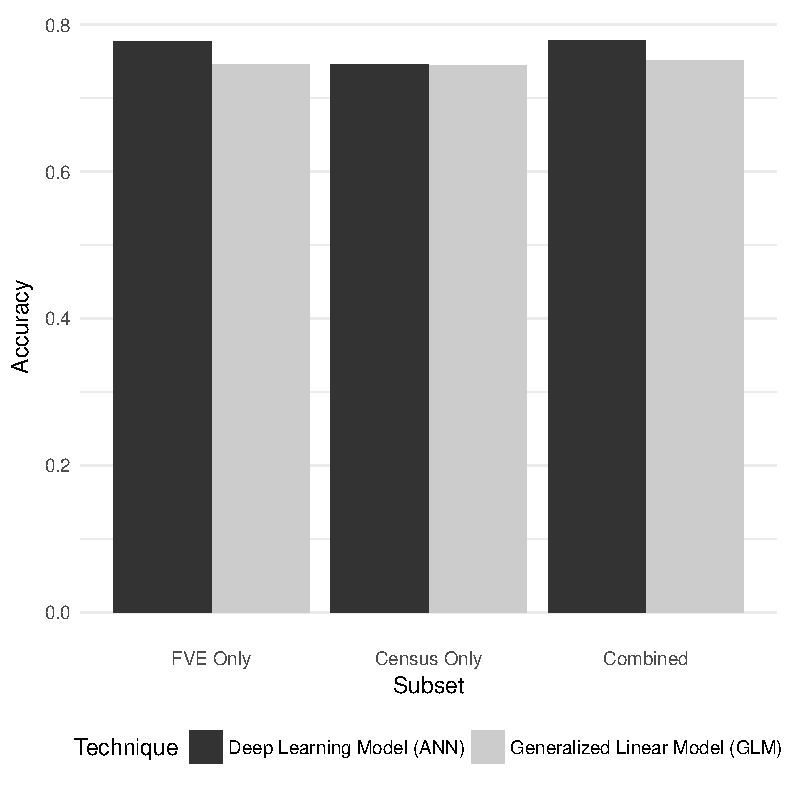
\includegraphics{Graphic003.pdf}
\end{figure}

\clearpage
\bibliography{Report}

\end{document}